% !TEX root = ./article.tex

\documentclass[spanish]{article}

\usepackage{mystyle}
\usepackage{myvars}
\usepackage{mylinearprogramming}



%-----------------------------

\begin{document}

	\maketitle % Insert title

	\thispagestyle{fancy} % All pages have headers and footers


%-----------------------------
%	ABSTRACT
%-----------------------------

	\begin{abstract}
		\noindent [TODO ]
	\end{abstract}

%-----------------------------
%	TEXT
%-----------------------------

	\section{Introducción}
	\label{sec:intro}

		\paragraph{}
		[TODO ]

		\subsection{Modelización Exacta}

			\paragraph{}
			[TODO ]

		\subsection{Heurística de Clarke y Wright}

			\paragraph{}
			[TODO ]


	\section{Resolución de Problemas}

		\subsection{Residuos}

			\paragraph{}
			[TODO ]

		\subsection{Gasóleos}

			\paragraph{}
			[TODO ]

		\subsection{E021-04m}

			\paragraph{}
			[TODO ]

			\begin{figure}[h]
				\centering
				\begin{subfigure}{.4\textwidth}
					\centering
					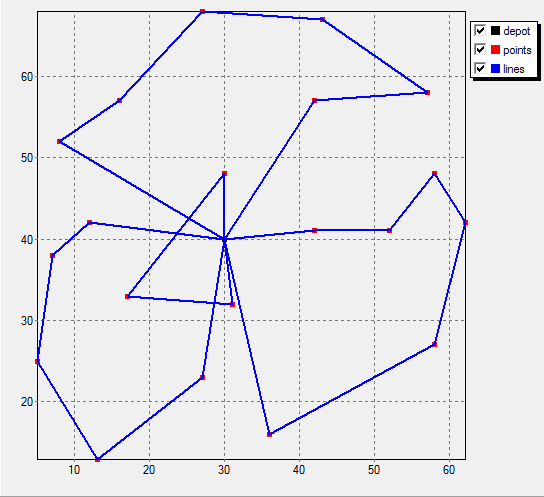
\includegraphics[width=\linewidth]{E021-04m-exact}
					\caption{Solución \emph{Exacta}}
				\end{subfigure} \
				\begin{subfigure}{.4\textwidth}
					\centering
					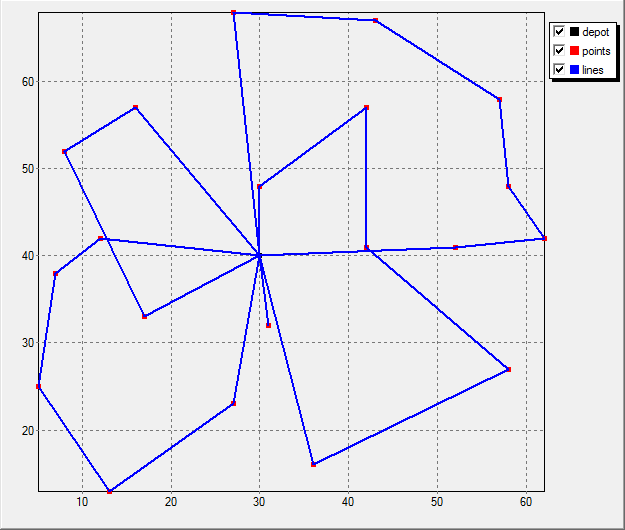
\includegraphics[width=\linewidth]{E021-04m-clarke-wright}
					\caption{Solución \emph{Clarke y Wright}}
				\end{subfigure}
				\caption{[TODO ]}
				\label{fig:sol-e021-04m}
			\end{figure}


		\subsection{E026-08m}

			\paragraph{}
			[TODO ]

			\begin{figure}[h]
				\centering
				\begin{subfigure}{.4\textwidth}
					\centering
					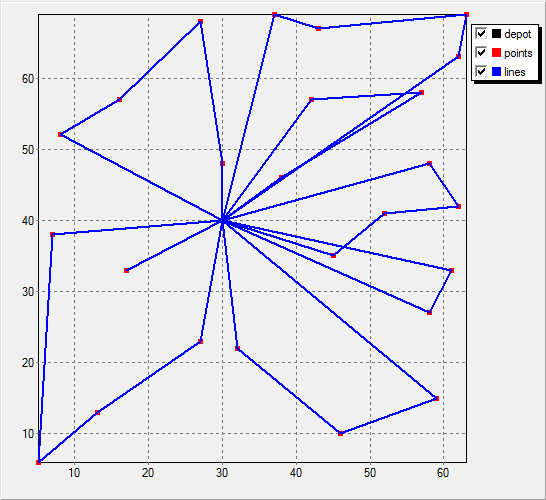
\includegraphics[width=\linewidth]{E026-08m-exact}
					\caption{Solución \emph{Exacta}}
				\end{subfigure} \
				\begin{subfigure}{.4\textwidth}
					\centering
					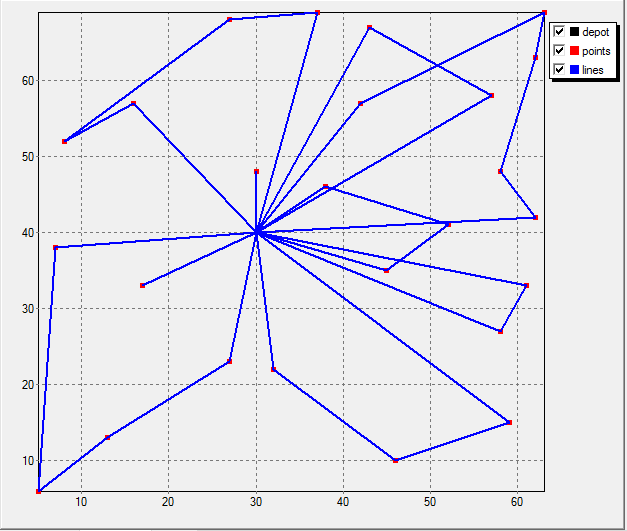
\includegraphics[width=\linewidth]{E026-08m-clarke-wright}
					\caption{Solución \emph{Clarke y Wright}}
				\end{subfigure}
				\caption{[TODO ]}
				\label{fig:sol-e026-08m}
			\end{figure}

		\subsection{E051-05e}

			\paragraph{}
			[TODO ]

			\begin{figure}[h]
				\centering
				\begin{subfigure}{.4\textwidth}
					\centering
					\includegraphics[width=\linewidth]{e051-05e-exact}
					\caption{Solución \emph{Exacta}}
				\end{subfigure} \
				\begin{subfigure}{.4\textwidth}
					\centering
					\includegraphics[width=\linewidth]{e051-05e-clarke-wright}
					\caption{Solución \emph{Clarke y Wright}}
				\end{subfigure}
				\caption{[TODO ]}
				\label{fig:sol-e051-05e}
			\end{figure}

		\subsection{E076-10e}

			\paragraph{}
			[TODO ]

			\begin{figure}[h]
				\centering
				\begin{subfigure}{.4\textwidth}
					\centering
					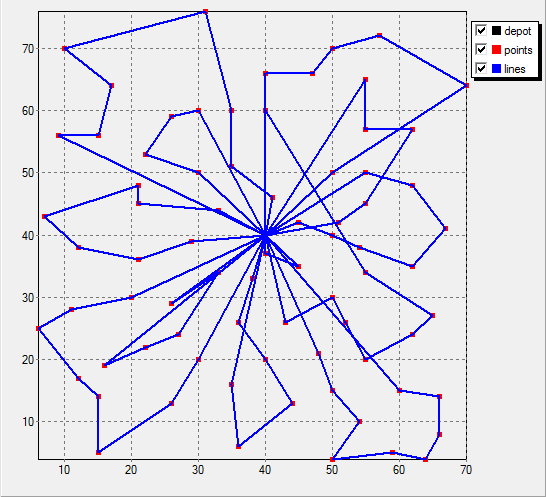
\includegraphics[width=\linewidth]{E076-10e-exact}
					\caption{Solución \emph{Exacta}}
				\end{subfigure} \
				\begin{subfigure}{.4\textwidth}
					\centering
					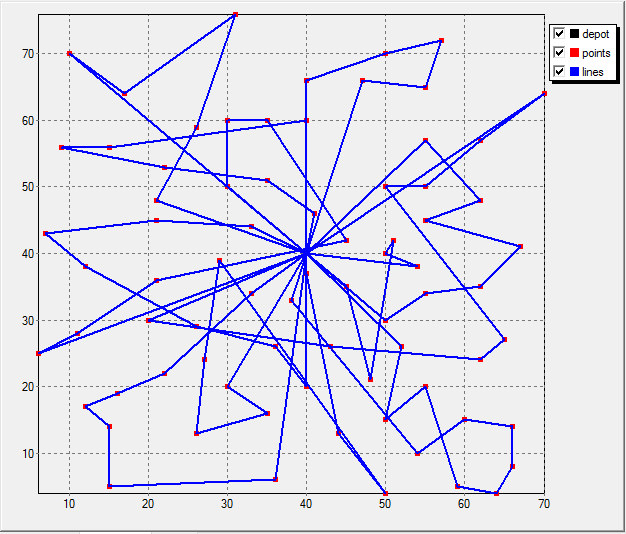
\includegraphics[width=\linewidth]{E076-10e-clarke-wright}
					\caption{Solución \emph{Clarke y Wright}}
				\end{subfigure}
				\caption{[TODO ]}
				\label{fig:sol-e076-10e}
			\end{figure}
%-----------------------------
%	BIBLIOGRAPHY
%-----------------------------
	\nocite{subject:mio}
	\nocite{garciparedes:mosel-examples}
	\bibliographystyle{acm}
  \bibliography{bib/misc}

\end{document}
